\section{Introduction to Mathematical Morphology}
\label{sec:introduction_to_mathematical_morphology}



\setcounter{subsection}{1}
\subsection{Erosion and Dilation}
% question 2 image:
\textbf{Question 1} \textit{Define erosion and dilatation from an ensemblist point of view and an functional point of view. Give some properties related to these operators.}



\textbf{Question 2} \textit{Operate in a binary image and a greyscale image with the MatLab commands imerode and imdilate. What are the effects on binary and grayscale images? Justify. Try with different structuring elements (different shapes, different sizes).}

In the figure below, the eroded and dilated images can be seen plotted next to the original image for each structuring element with the following shapes in order: rectangle, disk, diamond and line.

\begin{figure}[H]
    \centering
    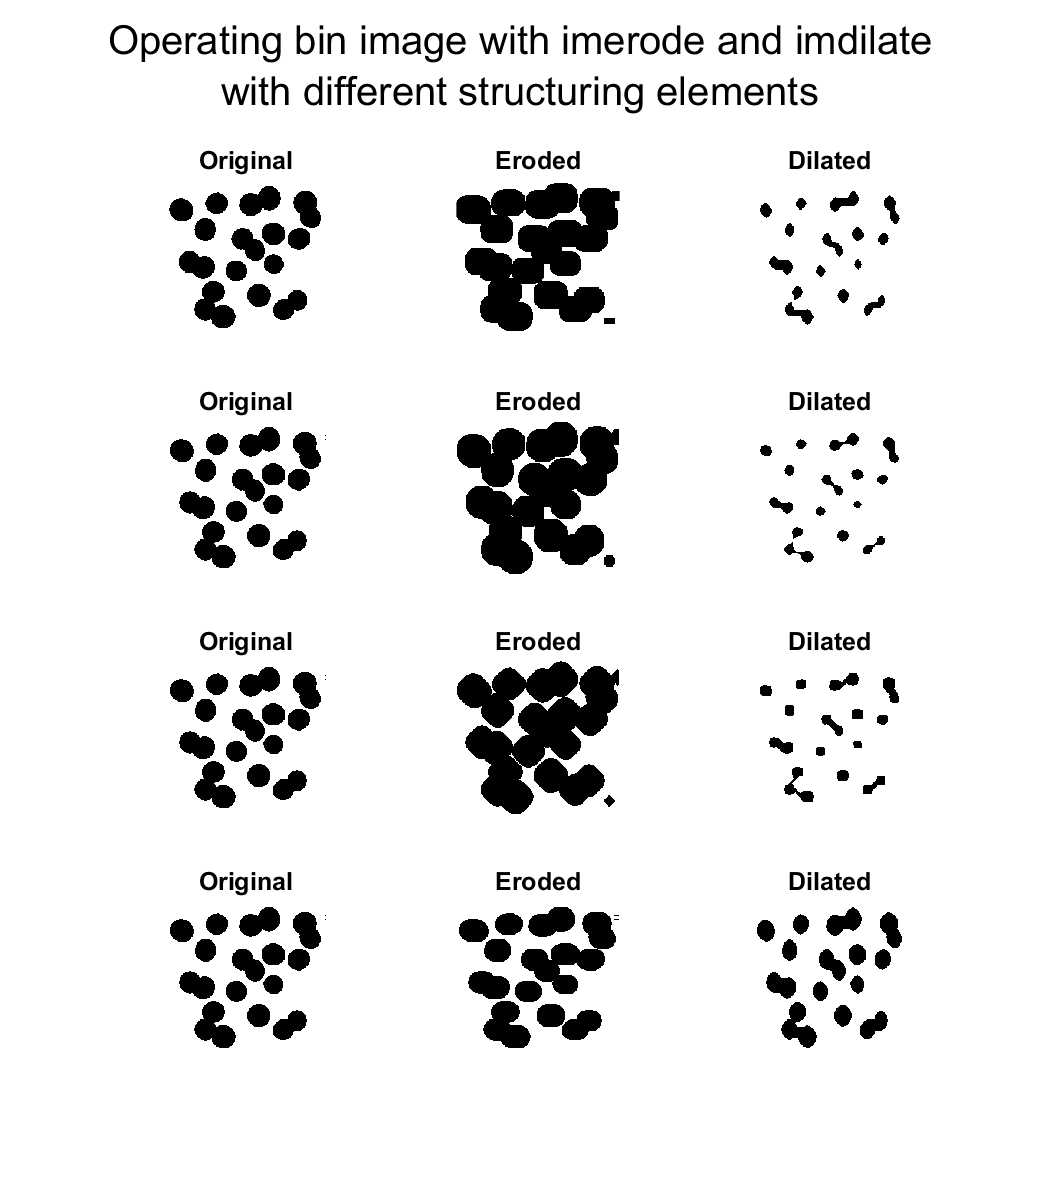
\includegraphics[width=0.8\linewidth]{Doc/Graphics/part2_Question2.png}
\end{figure}


\newpage
\textbf{Question 3} \textit{Extract internal and external edges of a binary image, and the morphological gradian.}
\begin{figure}[h]
    \centering
    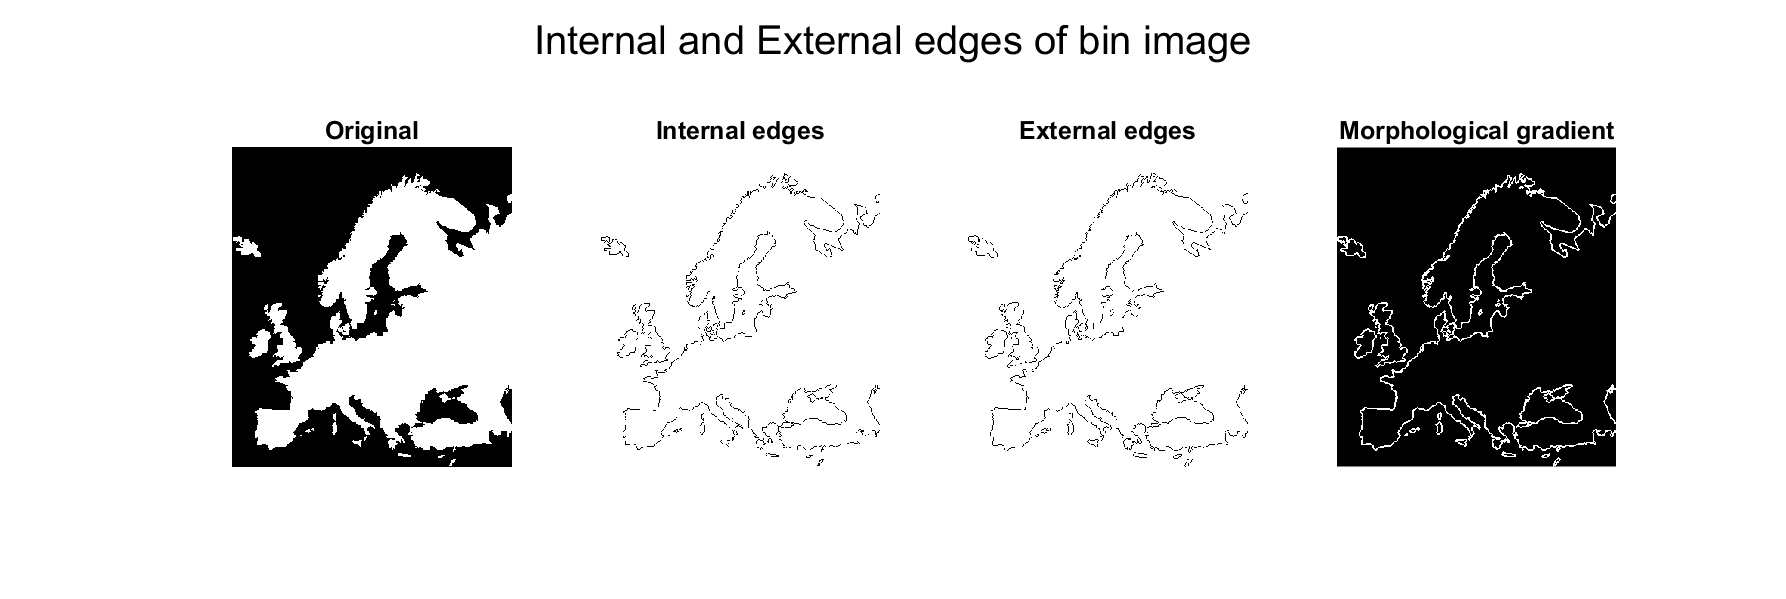
\includegraphics[width=1\linewidth]{Doc/Graphics/Part2_Question3.png}
\end{figure}


\textbf{Question 4} \textit{As an exercise, write an algorithm that show, in the map of Europe, the distance of each pixel w.r.t. the sea.}
\begin{figure}[h]
    \centering
    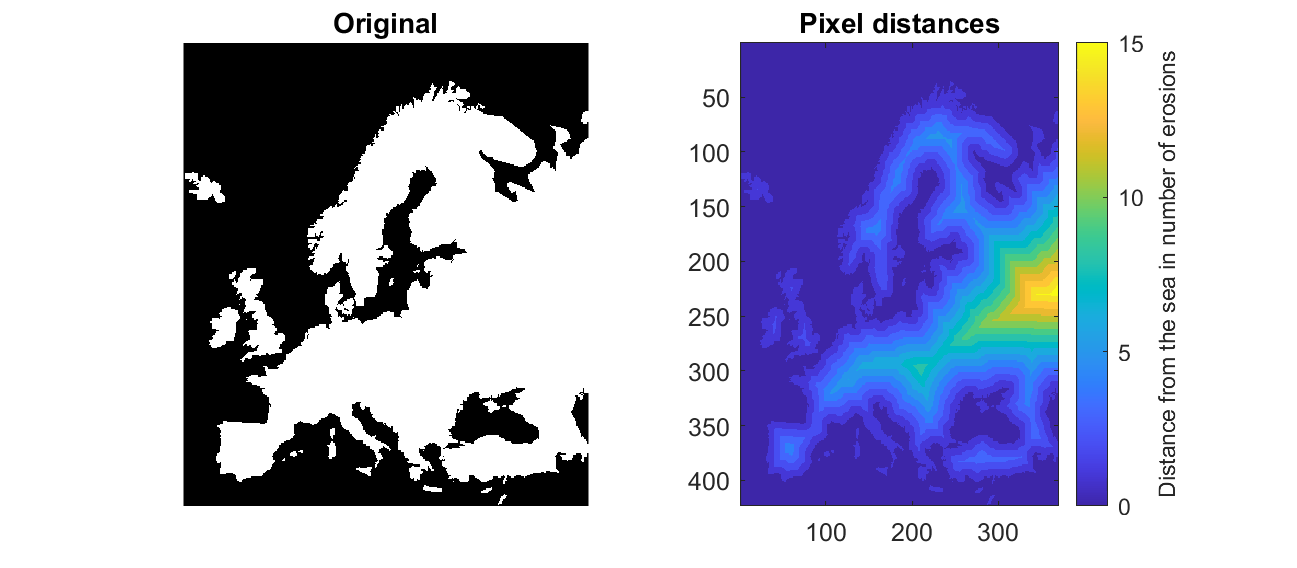
\includegraphics[width=0.75\linewidth]{Doc/Graphics/part2_Question4.png}
\end{figure}

\textbf{Question 5} \textit{Find an algorithm that detect rectangular objects of ’image2.jpg’.}

\textcolor{red}{TODO: Add pic from 5.}


\subsection{Morphological Filtering}
\subsubsection{Filters}
\textbf{Question 6} \textit{Define the two morphological filters called opening and closing. What are the effects on a binary image sur as ’image1.jpg’ (use the commands imopen and imclose)?}

\begin{itemize}
    \item \textbf{Opening filter:}
    some text

    \item  \textbf{Closing filter:}
    some text
\end{itemize}

\textcolor{red}{TODO: Add pic from 6}


\subsubsection{Form Detection}
\textbf{Question 7} \textit{The objective being to recognize some forms on images, find a simple algorithm to operate form detection}

See Question 5.


\textbf{Question 8} \textit{Apply a salt-and-pepper noise: what’s happen with your previous algorithm?}

The algorithm breaks and does not function at all due to the noise in the picture. See below:

\textcolor{red}{TODO add pic}

\subsubsection{Denoising}
\textbf{Question 9} \textit{Use the image Nebuleuse.jpg and apply a salt-and-pepper noise. De-noise the image by filtering.}

\textcolor{red}{TODO add pic}


\textbf{Question 10} \textit{Apply the same process to the ’Spain Beach’ image to isolate the beach itself.}

\textcolor{red}{TODO add pic}


\subsubsection{Top-Hat \& Black-Hat Filters}
\textbf{Question 11} \textit{Define op-hat and black-hat process in a 1D function: what is the associated process?}

\textcolor{red}{TODO Write shit here}


\textbf{Question 12} \textit{Define and operate top-hat and black-hat on a greyscale image. What do you observe?}

\textcolor{red}{TODO Write shit here}


\subsection{Morphological Skeletonization \& Segmentation}
\subsubsection{Skeletonization Process}
\textbf{Question 13} \textit{Write and operate a Skeletonization on the diplodocus.}
\textcolor{red}{TODO add pic}


\textbf{Question 14} \textit{Based on skelittization, find an algorithm that operate a segmentation in a binary image. Apply on ’image1.jpg’.}


\subsubsection{Image Segmentation}
\textbf{Question 15} \textit{Find a Skeletonization algorithm and operate on the Blood Cells image.}


